\documentclass[10pt,a4paper]{article}                        %format de page
\usepackage[utf8]{inputenc}                                                %encodage avec caractères accentués
\usepackage[T1]{fontenc}                                                %encodage
\usepackage[english,frenchb]{babel}                                                %typographie française
\usepackage{fancyhdr}
\usepackage{lastpage}
\usepackage{graphicx}
\usepackage{amsmath}
\usepackage{amsfonts,amssymb}
\usepackage{xcolor}
\usepackage{pict2e}

\usepackage{sidecap}
\usepackage{subcaption}

\usepackage{xcolor}
\usepackage{pict2e}
\usepackage{tikz} %Dessins

% Mise en page
\usepackage{geometry}
\geometry{a4paper,twoside,left=2.5cm,right=2.5cm,top=2.8cm,bottom=2.8cm} %taille et marges
\pagestyle{fancy}                                                                %style de page {fancy(package), empty, plain, headings}
\renewcommand{\headrulewidth}{0pt}                                %épaisseur du trait de tête de page (0.4pt)
\fancyhead[L]{}                                                                        %pied de page gauche
\fancyhead[C]{}                                                                        %pied de page centre
\fancyhead[R]{}                                                                        %pied de page droit
\renewcommand{\footrulewidth}{0pt}                                %épaisseur du trait du pied de page (0.4pt)
\fancyfoot[L]{}                                                                        %pied de page gauche
\fancyfoot[C]{}                                                                        %pied de page centrce
\fancyfoot[R]{\thepage{}/\pageref{LastPage}}        %pied de page droit

\thispagestyle{empty}                                % Page de garde vide

% Infos générales
\title{Symmetry Detection}
\author{Chantal DING, Chloé MACUR}
\begin{document}

\selectlanguage{english}

\thispagestyle{empty}							%page de garde vide
%\begin{document}
	\begin{center}
		\hfill
		Chantal \bsc{Ding}
		\hfill \hfill
		Chloé \bsc{Macur}
		\hfill ~
		\par
		\noindent
		\\
		\vspace{0.7cm}
		\textit{December 2013}
		\vfill\vfill
		\Huge
		\begin{tabular}{c}
			\hline
			%Projet\\
			{\Large{\textsc{Symmetry Detection}}}\\
			~~~A Planar-Reflective Symmetry\\ Transform for 3D Shapes~~~\\
			\hline
		\end{tabular}
		\large
		\vfill
		 Project report\\
		 INF555 -- Digital Representation and Analysis of Shapes
	\end{center}
	\vfill
	\begin{flushright}
	
\includegraphics[scale=0.1]{img/logo_x_h.jpg}
	\end{flushright}
	\newpage 
\newpage
\tableofcontents

\newpage
        
        \section*{Introduction}
\addcontentsline{toc}{section}{Introduction}
  
        A lot of 3D shapes, whether natural or man-made, present some kind of symmetry that can be really useful in computer vision and 3D geometry.  Indeed symmetries allow certain economy, especially in digital representation, but they are also involved in pattern recognition or geometry completion. Thus, numerous methods are used to detect symmetries, partly because of the diversity of datas (point clouds, polygon meshes, NURBS, patches, etc.).  
 
        \section{A Planar-Reflective Symmetry Transform for 3D Shapes}
        
        We chose to try to implement the planar reflective symmetry transform (PRST) described by Podolak et al.~\cite{Podolak:2006:APS}. This transform takes a 3D shape and aims at getting the space of planes that are associated to a reflectional symmetry. It provides both global symmetries, certain local symmetries and even imperfect symmetries. Moreover, it is not sensitive to noise or missing data. For a proper understanding of this method, we transcribe here some of the formulas used.\\
        
        Given a function $f$ representing the energy, $PRST(f,\gamma)$ is a measure of $f$'s symmetry with respect to the plane reflection $\gamma$.
        The symmetry distance, $SD(f,\gamma)$ is defined as the $L_2$ distance between $f$ and the nearest function that is invariant to that reflection:
        \begin{displaymath}
        SD(f,\gamma) = min_{g|\gamma(g)=g} \lVert f-g \lVert . %TODO afficher en dessous
        \end{displaymath}

Which leads, by normalizing the symmetry measure, to
$$ PRST^2(f,\gamma) = 1 - \frac{SD^2(f,\gamma)}{\lVert f \lVert ^2}         $$

However, the nearest symmetric function to $f$ is the average of $f$ and $\gamma(f)$:
$$ SD(f,\gamma) = \lVert f - \frac{f + \gamma(f)}{2} \lVert = \frac{\lVert f - \gamma(f) \lVert }{2} $$

Therefore, we have:
$$ PRST^2(f,\gamma) = 1 - \frac{SD^2(f,\gamma)}{\lVert f \lVert ^2} =  1 - \frac{\lVert f - \gamma(f) \lVert ^2 }{4 \lVert f \lVert ^2}        =  1 - \frac{\lVert f \lVert ^2 - 2f.\gamma(f) + \lVert \gamma(f) \lVert ^2 }{4 \lVert f \lVert ^2} $$

If $f$ is normalized\footnote{We will discuss that point in \ref{comments}}, we obtain
\begin{equation}
PRST^2(f,\gamma) = \frac{1 + f.\gamma(f)}{2}
\label{equation_simplifiee}
\end{equation}

        Thus, to evaluate the symmetry measure for a plane, we need to evaluate the following estimator, called Monte Carlo estimator :
$$ D(f,\gamma) = f.\gamma(f). $$
        
        To compute this PRST we chose to use a Monte Carlo algorithm, which computes a discrete version of the PRST that takes advantage of sparsity in the function $f$. This sparsity is mostly found in  point sets and rasterized surfaces.
        The brute force approach would be to evaluate the PRST for every single plane in the space of the figure. That would be done by selecting a pair of points and voting for the plane between them. Instead of chosing the points randomly, we favour the points corresponding to a high energy of function $f$.\\
        

\indent \indent \textbf{for} sampled points $x$:\\
\indent \indent \indent \textbf{for} sampled points $x'$: \\
\indent \indent \indent \indent $\gamma \leftarrow$ reflection plane($x, x'$)\\
\indent \indent \indent \indent $D(f,\gamma) += w(x, x',\gamma).f(x).f(x')$\\
        
Moreover we do not vote for planes but discretized bins of planes and we weight the vote of each pair of points:
$$ w(x, x',\gamma) = w_{samp} . w_{change-of-variables} $$

$w_{samp}$ is the reciprocal of the probability of having selected the two points :
$$w_{samp}(x, x',\gamma) = \frac{1}{f(x).f(x')}. $$

The $change-of-variables$ is due to the fact that we move from a pair of points to discretized bins represented by polar coordinates. In 3D spherical coordinates, it is given by the formula \[w_{change-of-variables} = 2d^2\sin\theta\]
where $\theta$ is the angle of the bin from the origin.\\

This leads to $$ w(x, x',\gamma) = \frac{1}{f(x)f(x')2d^2\sin\theta}. $$

In the end, we obtain
\begin{equation}
D(f,\gamma) = \frac{1}{N_{samp}} \sum_{i=1}^{N_{samp}}\frac{1}{2d^2\sin\theta}
\label{equation_finale}
\end{equation} 

        
        \section{Our implementation}

        \subsection {Conventions and Notations}
We chose to use classic image formats (png, jpg) as input files as they are naturally rasterized. For more simplicity we only considered grayscale images. Since the method we are implementing is taking advantage of sparsity in the function, a typical input image would be a black and white outline (see Figure \ref{exemple_carre}). The Java class \texttt{BufferedImage} provides an easy way to access such images and manipulate them as arrays of integers between 0 and 255. 
\begin{figure}[h]
\begin{center}

\includegraphics[scale=0.5]{img/carre.png}
\caption{Example of input image}
\label{exemple_carre}
\end{center}
\end{figure}

Since pixel values are high for white and low for black, we want to work with the function $f$ defined as follows for each pixel $p$ of the image $I$ :
\[f(p) = 255 - \text{intensity of $I$ at $p$}\]
so that $f(p)=0$ for white pixels, i.e. empty space.

For point coordinates, we simply use the default Java coordinate system, with $(0,0)$ in the upper-left corner, as shown in Figure \ref{coordinates}. All points have integer coordinates. Lines however, are parametrized over a pair of \texttt{double} values $(r,\theta)$ where $|r|$ is the distance of the line to the origin and $\theta$ the angle of the normal vector, as shown in Figure \ref{lines_parametrization}. In order to easily retrieve $\theta$ from $\sin\theta$, we chose to have $\theta\in\left]-\frac{\pi}{2},\frac{\pi}{2}\right]$ and the radius $r$ can be negative.


\begin{figure}[h]
\begin{center}
\begin{picture}(150,110)
\put(10,105){\vector(1, 0){90}}
\put(10,105){\vector(0, -1){90}}
\put(0,110){$(0,0)$}
\put(105,105){$x$}
\put(5,5){$y$}
\put(15,15){
\includegraphics[scale=1.8]{img/a.png}}
\end{picture}
\end{center}

%\begin{figure}[h]
%\begin{center}
%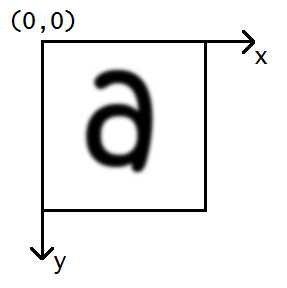
\includegraphics[scale=0.5]{img/coordinates.png}
%\caption{$(x,y)$ coordinates for Java images}
%\label{coordinates}
%\end{center}
%\end{figure}
\caption{$(x,y)$ coordinates for Java images}
\label{coordinates}        
\end{figure}

\begin{figure}[h]        
\begin{center}
\begin{picture}(250,110)
\put(10,105){\vector(1, 0){190}}
\put(10,105){\vector(0, -1){90}}
\put(0,110){$(0,0)$}
\put(205,100){$x$}
\put(10,5){$y$}
\textcolor{blue}{\put(0,40){\line(5,2){200}}}
\put(31,52){\line(-2,5){21}}
\put(20,60){$r$}
\qbezier(15,90)(25,100)(25,105)
\put(16,91){\vector(-1, -1){1}}
\put(25,90){$\theta$}
\end{picture}
\end{center}

%
%\begin{figure}[h]
%\begin{center}
%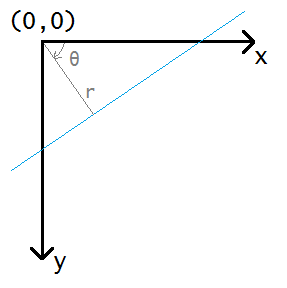
\includegraphics[scale=0.7]{img/lines.png}
%\caption{$(r,\theta)$ parametrization of lines}
%\label{lines_parametrization}
%\end{center}
%\end{figure}        
\caption{$(r,\theta)$ parametrization of lines}
\label{lines_parametrization}
\end{figure}

        \subsection{Sampling}
In order to compute the PRST using the Monte Carlo algorithm for sparse functions, we first perform an importance sampling of points in the image, using $f(x)$  as the probability density of selecting $x$. For this, we use the cumulative sum of $f(x)$ over the image as the cumulative distribution function and perform an inverse transform sampling. Usually, this method works by generating a real number $u$ in range [0,1] and computing $F^{-1}(u)$, where $F$ is a cumulative distribution function. Here, we adapted the method to work with non-normalized integer functions :
\begin{enumerate}
\item Generate a random integer n in range $[0,max_F]$, where $F$ is the cumulative sum of pixel values and $max_F$ its maximum value;
\item Let $p_1,...,p_N$ be the pixels of the image, compute $i=\inf\{m\in \mathbb{N}, m\leq N |  F(p_m) = n\}$;
\item Add $p_m$ to the sample.
\end{enumerate}



        \subsection{Adjustments for 2D}
        

The Monte Carlo algorithm we chose to use for computing the PRST requires to derive a change-of-variable weight for each pair of points $(x,x')$, accounting for the transformation between the discrete parametrization of lines over $(r,\theta)$ and the pairs of reflected points. In 3D, the change-of-variables weight is given by the following formula :
\[w_{change-of-variables} = 2d^2\sin\theta\]
However, since we are working in 2D, we need to recompute this weight in order to fit the new coordinates system. As in 3D, we compute the determinant of the Jacobian of the change-of-variables transformation. Let 
\[\vec{n}=\begin{pmatrix}\cos\theta \\ \sin\theta\end{pmatrix}\]
be the normal of the axis of reflection, $d$ the distance between $x$ and $x'$, we can write :

\begin{SCfigure}
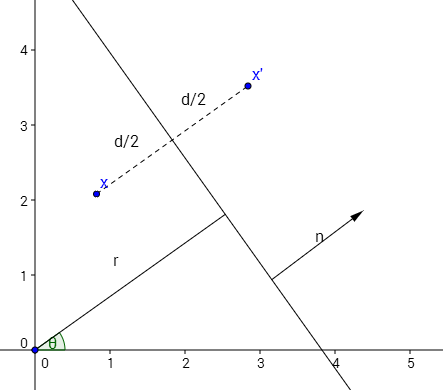
\includegraphics[scale=0.6]{img/definitions.png}
\caption{cartesian and polar coordinates}
\label{definitions}
\end{SCfigure}

\begin{align*}
 d & = \lVert x-x' \rVert  \\
& = 2(r-\vec{n}\cdot x) \\
x' &= x+ d\vec{n}\\
&= x+ 2(r\vec{n} - (\vec{n}\cdot x)\vec{n})
\end{align*}
thus we have :
\begin{align*}
\frac{\partial x'}{\partial r}&=2\vec{n}\\
\frac{\partial x'}{\partial \theta}&= 2r\vec{u}-2[(\vec{u}\cdot x)\vec{n}+(\vec{n}\cdot x)\vec{u}]
\end{align*}
where 
\[\vec{u}=\frac{\partial \vec{n}}{\partial \theta} = \vec{n}=\begin{pmatrix}-\sin\theta \\ \cos\theta\end{pmatrix}.\]
Therefore, the Jacobian is
\[J = 2
\begin{pmatrix}
\cos\theta & -r\sin\theta-(\vec{u}\cdot x)\cos\theta+(\vec{n}\cdot x)\sin\theta\\
\sin\theta &  r \cos\theta - (\vec{u}\cdot x)\sin\theta - (\vec{n}\cdot x)\cos\theta
\end{pmatrix}\]
and so the determinant is
\[w_{change-of-variables} = |J| = 2d.\]

We were initially suprised by the lack of dependence in $\theta$, contrary to the 3D formula given in the paper. However, noting that the cartesian-to-polar (2D) and cartesian-to-spherical(3D) change-of-variables jacobian determinants are respectively given by \[|J_{cartesian-to-polar}| = r=\frac{w_{2D-change-of-variables}}{2}\] and \[|J_{cartesian-to-spherical}|=r^2\sin\theta=\frac{w_{3D-change-of-variables}}{2}\] gives a good intuition on why there is such a descrepancy between the 2D and 3D weights. Finally, the 2D Monte Carlo estimator is given by :\[D(f,\gamma) = \frac{1}{N_{samp}} \sum_{i=1}^{N_{samp}}\frac{1}{2d}.\]


          \subsection{Comments}
          \label{comments}
          The value $N_{samp}$ used in formula~\eqref{equation_finale} is not clearly defined. We find it not consistent that it is both the normalization factor and the terminal of the sum. This normalization of $f$ may used to obtain equation ~\eqref{equation}. In that case, the terminal of the sum would be the number of pairs that voted for the bin and not the total number of points.\\
          
          Bounds : la valeur du prst (monte carlo) obtenue telle qu'on le fait dépend complètement de l'unité de longueur qu'on utilise pour calculer les distance x,x'. Du coup on n'a vraiment aucune garantie sur les bornes du prst Monte Carlo, contrairement au prst complet...\\
          
        The PRST obtained by Monte Carlo algorithm seems to depend on the unit chosen. The way we calculated it -- using a pixel as a unit -- the Monte Carlo indicator $D$ is  between 0 and 1 but it was implicit. Thus, if we calculate $PRST^2(f,\gamma) = \frac{1 + D(f,\gamma)}{2}$ the bounds are not 0 and 1, which is why we used D as if it was PRST. Beyond this issue, we have very low values in any case.
          
          
          \section{Results}

We visualized the computed PRST applying a treashold proportional to the maximum PRST value, and tracing the lines corresponding to the strongest symmetries. The lines are traced in colors ranging from blue to red, with red for the stronger symmetries and blue for the weaker ones. We used an alpha channel to add transparency to the lines and allow the original image to show through, as well as making areas with high density of lines more legible. Figure \ref{visualization} shows a few examples of computed PRST.

\begin{figure}[h]
        \centering
        \begin{subfigure}{120 pt}
                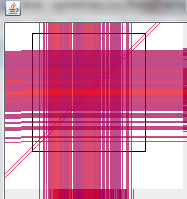
\includegraphics[height=120 pt]{img/carre2_5000.png}
                \caption{square}
                \label{square}
        \end{subfigure}
        ~
        \begin{subfigure}{120 pt}
                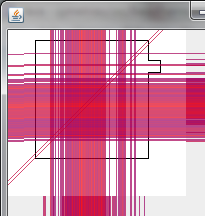
\includegraphics[height = 120pt]{img/carre3_5000_bis.png}
                \caption{bumped square}
                \label{bump_square}
        \end{subfigure}
       
       ~\\
        \begin{subfigure}{120 pt}
         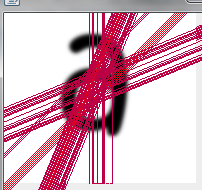
\includegraphics[height=120 pt]{img/sample_1000_seuil_07.png}
         \caption{the letter a}
                \label{a}
                   \end{subfigure}
        ~
        \begin{subfigure}{120 pt}
         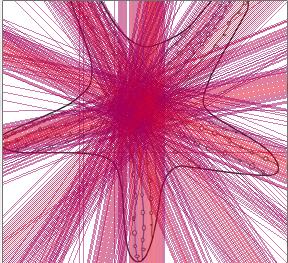
\includegraphics[height=120 pt]{img/n_32_sample2000_seuil06.png}
         \caption{a starfish}
                \label{star}
              \end{subfigure}     
                \caption{Visualizations of the PRST for several 2D outlines}
        \label{visualization}
\end{figure}

One of the main claims of PRST is its stability and insensibility to noise. We empirically tested the claim by comparing the PRST visualization of a square and a modified version of the square with a small bump added to the outline. As can be seen in Figure \ref{square} and Figure \ref{bump_square}, the two inputs yield similar results. The PRST is also good at detecting approximate symetries, and we had fairly good results with the image of a starfish (Figure \ref{star}).

\begin{figure}[h]
\centering
 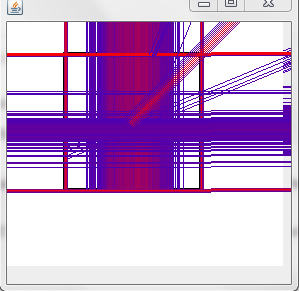
\includegraphics[scale = 0.7]{img/n_16_sample_1000.png}
 \caption{Example of "overbearing" local symetries}
 \label{thick_square}
\end{figure}

However, our implementation presents a few weaknesses. Some local symetries appear with too much emphasis, in particular for input images containing thick straight lines. Figure \ref{thick_square} gives a good example of the phenomenon : the local symetries of the four sides of the squares appear to have a higher PRST than the main axis of symetry. We believe it is due to the $\frac{1}{2d}$ term in $D(f,\gamma)$ giving too much importance to local symetries in dense areas. The phenomenon persists even with a sampling size as high as 10,000 points, suggesting that sampling size is unable to compensate for the weight given to closer pairs of points.

The threashold method for visualizing the PRST is also imperfect. In order to obtain legible results, we need to tweak the threashold value for every change of input image or sample size. Despite the $\frac{1}{N_{samp}}$ normalization, there is no "universal" threashold one can use to discriminate strong symetries from weak symetries in an image. For input images containing numerous axes of symetry, this results in difficult to read visualization (see Figure \ref{rosace}, since a high number of axes will have a PRST value close to the maximum. Figure \ref{rosace 2} shows that using a higher threashold does not give better results.

\begin{figure}[h]
\centering
 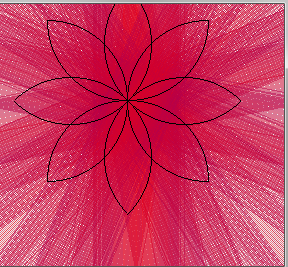
\includegraphics[scale = 0.7]{img/rosace_5000.png}
 \caption{Visualization of PRST values of an image with a high number of symmetries}
 \label{rosace}
\end{figure}


\begin{figure}[h!]
\centering
 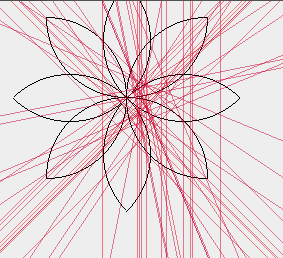
\includegraphics[scale = 0.7]{img/rosace_2000_seuil08.png}
 \caption{Visualization of PRST values of an image with a high number of symmetries, with a threashold of $0.8max$}
 \label{rosace 2}
\end{figure}

        \section*{Conclusion}
\addcontentsline{toc}{section}{Conclusion}
We have implemented the Monte Carlo algorithm to calculate a discrete version of the planar reflective symmetry transform for 2D shapes, by adapting the 3D method in 2D. We managed to perform an efficient sampling according to the density of points in the image. Then we selected pairs of sampled points and voted for the most accurate bin of planes between them. In our values we obtain some outliers, given that the PRST values are unevenly distributed in $[0,1]$ and that bold edges happend to be too thick and symmetrical, which can creates disturbances. However, we managed to obtain good results namely high PRST values corresponding to symmetry axes in the original picture. As a result, we measured the symmetry of an object with respect to all planes in a discrete space. Computer graphics benefit from that type of symmetry information, which allows a certain efficiency and economy in shape processing.

\addcontentsline{toc}{section}{References} 
\nocite{*}
\bibliographystyle{plain}
\bibliography{bibli}
                
\end{document}